


    %\section{Gravitational waves in astrophysics}
    %\label{grav_waves_astro}

        Space should reverberate with gravitational waves. 
Light shows part of cosmic history; now, primeval epochs and secret stellar reaches might be seen in patterns of light transformed by gravity. 
General Relativity and related theories of gravitation posit~\cite{EinsteinRosen1937} that changing quadrupolar masses radiate gravitationally, just as accelerating dipolar charges do electromagnetically. 
In those waves we might see black holes and neutron stars colliding, supernovae, the dawn of the Big Bang and rotating neutron stars -- and the potential for unanticipated insights, into other objects or laws of physics, is too tantalizing to ignore. 
As yet, we have made no direct detections. 
Hulse and Taylor \cite{HulseTaylor1975} observed a neutron star in a binary system, PSR 1913+16, with an orbit shrinking just as gravitational radiation would predict. 

Following on the pioneering work of Joseph Weber with bar detectors~\cite{Weber1960} and Robert Forward with tabletop interferometers~\cite{Forward1978}, kilometer-scale interferometers were built at the end of the last millenium to look for gravitational radiation. 
Laser light in these instruments travels orthogonal paths and is reflected back; shifts in the combined pattern are scrutinized for indications that gravitational waves stretched space itself. 
LIGO (the Laser Interferometer Gravitational-wave Observatory)~\cite{LIGOFirst2004,Fricke2009}, Virgo~\cite{Acernese2005}, and GEO600~\cite{Willke2002,Hild2009}, soon to be joined by KAGRA~\cite{Kuroda2010}, are kilometer-scale intereferometers, gravitational wave antennae standing on the threshold of discovery.
This thesis includes analysis of LIGO data.

Vibrations in spacetime's metric require many steps to detect.
The author's work has pursued a series of clearer perspectives on detection: filtering \& regressing out correlated noise, helping cancel fluctuations in the electromagnetic field with quantum optics, and looking for continuous waves from promising neutron stars in binary systems. 
Chapter~\ref{chap2} describes General Relativity's prediction of gravitational waves and the design \& operation of LIGO.
Noise intrinsic to the optical configuration of these instruments is subtracted post-facto by feedforward filtering using recorded servo data in Chapter~\ref{chap3}. 
Quantum optical squeezing reduces relevant uncertainties per Heisenberg's principle in Chapter \ref{chap4}.
Then the search begins.
Astrophysicists expect to find signals from four categories of cosmic sources: inspiralling binary systems of stellar remnants, supernovae and similar bursts, stochastic background, and continuous waves from neutron stars.
Einstein's theory predicts the intensity, speed, and polarization of gravitational waves that could be emitted from these sources.
Low-mass X-ray binaries (LMXBs) should lead astronomically long lifetimes, radiating continuous waves from their constituent neutron stars.
Chapters \ref{chap5} and \ref{chap6} use these expectations to enhance and run Fourier-domain analyses of simulated and real data.
These searches target the LMXB Scorpius X-1 and X-ray transient J1751-305.
Astronomy has grown from humanity's first glimpses into the night sky with the unaided eye. 
With every new instrument, from Galileo's telescope through radio antennae and neutrino catchers, our understanding of the cosmos has grown. 
Communicating that understanding is the subject of Chapter \ref{chap7}.
Gravity pervades the universe like no other force: we must hear its tale. 
        
%This thesis describes efforts to make that search more sensitive with quantum optics at the observatories, by filtering noise from the data, and by conducting a promising search for continuous waves from neutrons stars in binary systems.

\begin{figure}
\begin{center}
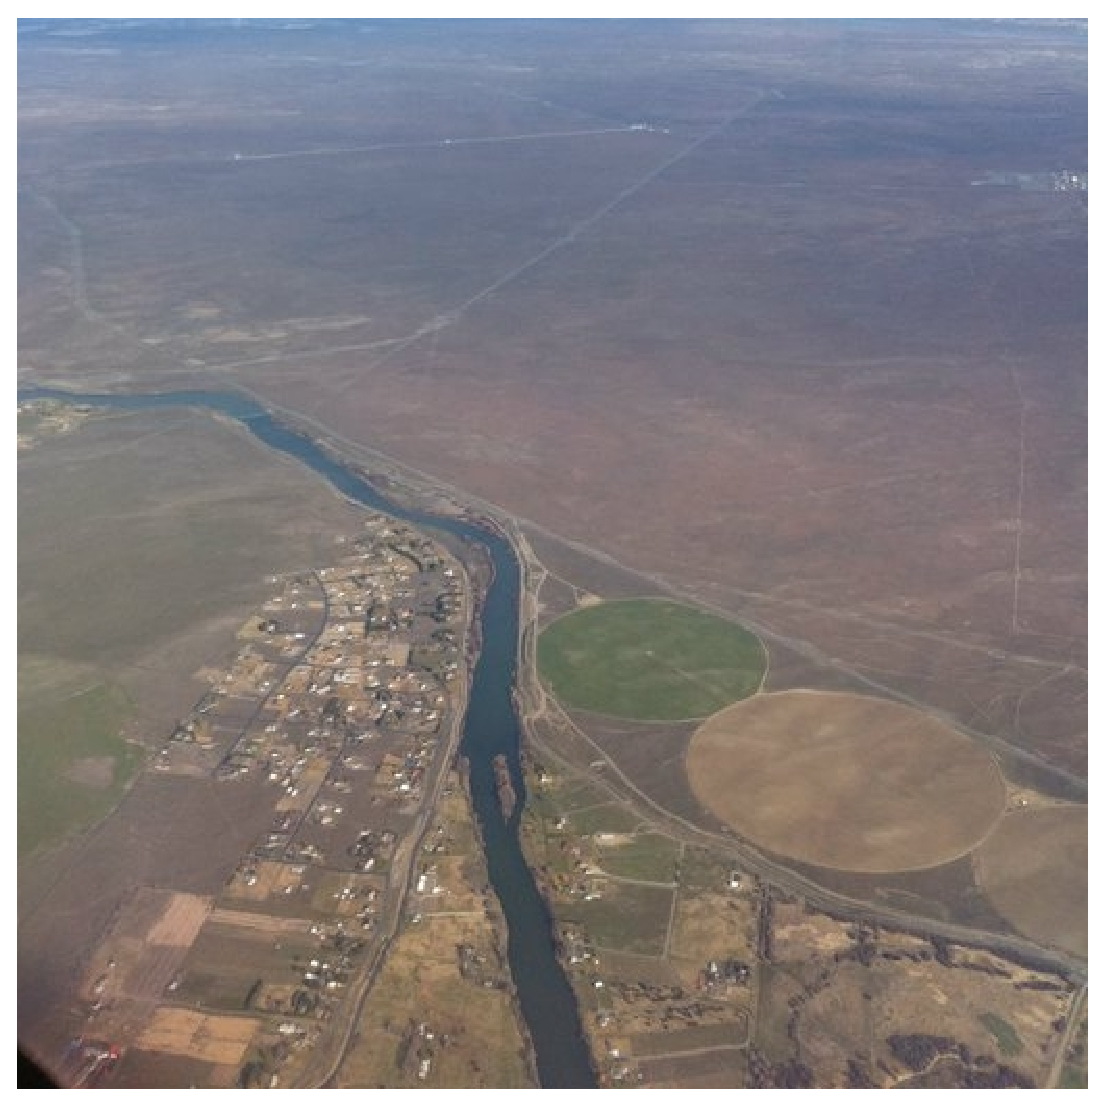
\includegraphics[keepaspectratio=true,scale=0.75]{plots/frontispiece/LIGO_Hanford_Observatory_from_above_Rattlesnake-small.eps} 
\caption{
LIGO Hanford Observatory, at top in the plain in this north-looking photograph.
Hanford Route 10 passes closest to the corner station joining the arms. 
Highway 240 goes northwest. 
The Yakima River flows southwards, joining the Columbia River downstream.
}
\end{center}
\end{figure}

\begin{figure}
\begin{center}
\includegraphics[keepaspectratio=true,scale=0.3]{plots/frontispiece/View-of-LIGO-aerial-small.eps} 
\caption{
View closer to LIGO Hanford Observatory. 
Ripples in the plain catch wind.
The corner station connects the X and Y arms, 4 kilometers long, which each have a mid- and end-station. 
The corner station also contains the laser, beam-splitter, and photo-detector of the gravitational wave interferometer.
}
\end{center}
\end{figure}
            
%        --------------------
%
%	Here is a sample chapter file. The chapters of the thesis
%	should be saved to seperate files such as
%	\textit{chapter1.tex}. In the file \textit{thesis.tex} the
%	\textit{input} command then includes these chapters into the
%	thesis. Note that none of the chapter files need any headers.
%	This header for each of these files is contained in
%	\textit{thesis.tex}. The file \textit{thesis.tex} also
%	includes the numbers system for the sections, figures,
%	theorems lemmas etc...

%\section{Sample Section}
%\label{sample_section}
%
%	This is what a sample section looks like. Let's conclude this
%	section with a sample theorem statement and proof.
%
%	\begin{theorem}
%	\label{sample_theorem}
%	The are an infinite number of prime numbers
%	\end{theorem}
%
%	\emph{Proof:} On the contrary assume there are a finite number
%	of primes $P_1, P_2, ... P_n$. Consider $\mathcal{P} = P_1 P_2
%	\cdots P_n+1$. $\mathcal{P}$ is not divisible by any of the
%	primes in our finite set. (Contradiction) $\square$
  

